\chapter{System Configuration}
\label{ch:system_configuration}

This chapter describes the physical configuration of the LINKU satellite system. The operational configuration names introduced in Chapter~\ref{ch:mission_overview_conops} are used here to describe the corresponding satellite accommodation, geometric envelopes, and deployment interfaces.

The LINKU system follows a carrier--payload architecture composed of SAT-A, SAT-B, and SAT-C. SAT-A is the carrier satellite and provides the external CubeSat-compatible structure for accommodating the tether-experiment payload. SAT-B and SAT-C form the coupled SAT-BC assembly before internal separation and become the two end bodies of the tethered system after the SAT-B/SAT-C separation command.

SAT-A is based on a 12U CubeSat-compatible configuration. Its main role is to accommodate, protect, and release the SAT-BC assembly once the required deployment conditions are met. For this purpose, SAT-A includes an ejection platform located below the SAT-BC assembly. The release path is directed through the upper section of SAT-A, while the SAT-A bus subsystems are allocated in the lower region of the satellite. This arrangement preserves the upper volume for the tether-experiment payload and separates the carrier functions from the SAT-B/SAT-C experiment hardware.

The SAT-A configuration also provides the satellite functions required before SAT-BC release, including onboard computing, electrical power, communications, attitude determination and control, and power generation. These functions support the stabilization and orientation of the integrated SAT-ABC configuration before payload release. Detailed subsystem implementations are described in the corresponding satellite subsystem sections.

SAT-B is the main satellite of the tether experiment. It uses a non-standard small-satellite geometry, with an external envelope that can be approximated by an equivalent diameter of approximately \(20~\mathrm{cm}\). The current reference mass estimate for SAT-B is approximately \(5~\mathrm{kg}\). Unlike SAT-A, SAT-B does not follow a conventional CubeSat form factor, since its geometry is driven by the tether storage, SAT-C accommodation, and deployment-interface requirements. SAT-B accommodates the tether storage and deployment elements, the SAT-B/SAT-C separation interface, experiment electronics, communications equipment, and the measurement interfaces required to observe the tethered-system response.

SAT-C is the second end body of the tethered system. It also uses a non-standard small-satellite geometry, with an external envelope that can be approximated by an equivalent diameter of approximately \(10~\mathrm{cm}\). The current reference mass estimate for SAT-C is approximately \(0.5~\mathrm{kg}\). SAT-C carries the local instrumentation associated with the tether end, including the elements required for imaging, relative-position measurement, and tether-tension sensing. SAT-C does not include a dedicated active ADCS; after separation, its motion is governed by the tether interaction and the overall tethered-system dynamics.

Before SAT-B/SAT-C separation, SAT-B and SAT-C remain mechanically coupled as the SAT-BC assembly. In this configuration, SAT-C is partially accommodated within the upper region of SAT-B. This arrangement is driven by the height constraint imposed by the SAT-A internal accommodation volume. The SAT-BC assembly is therefore treated as a coupled payload before internal separation and as the deployable tether-experiment system after release from SAT-A.

Figure~\ref{fig:linku_project_mechanical_layout} shows the mechanical layout of the SAT-ABC integrated configuration. The figure illustrates the location of the SAT-BC assembly inside SAT-A, the ejection platform below the payload, and the lower region reserved for the SAT-A bus subsystems.

\begin{figure}[htbp]
    \centering
    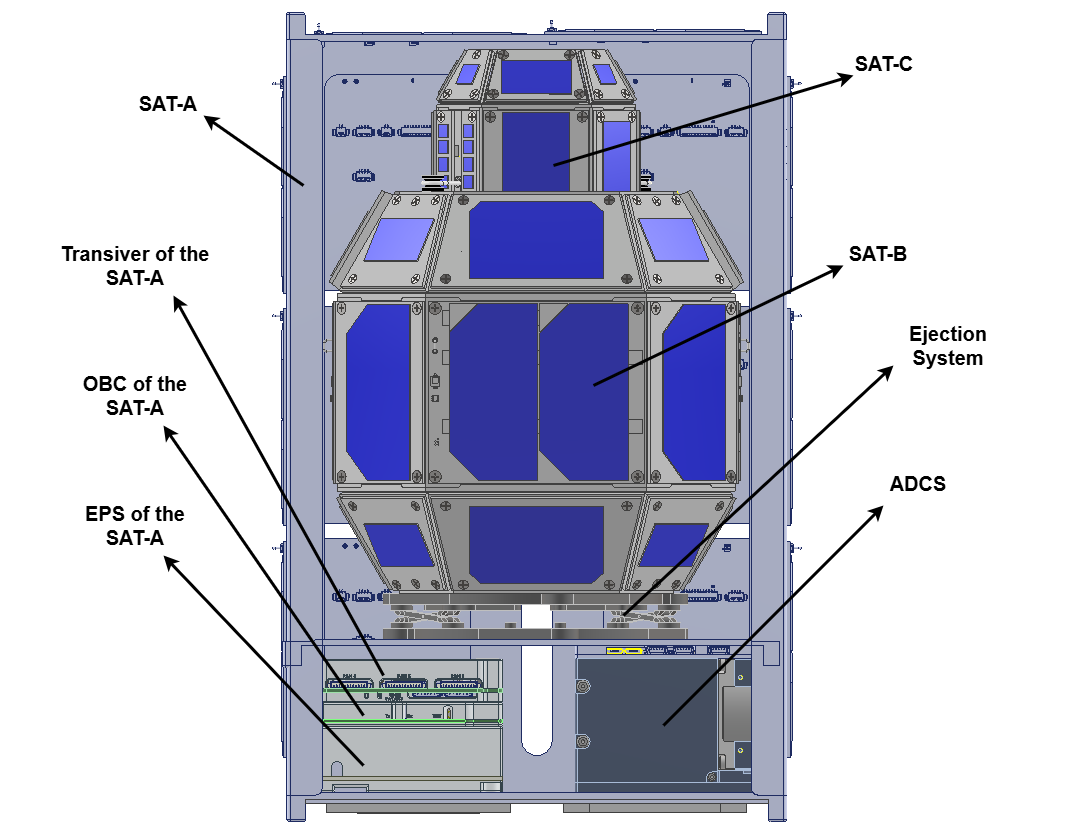
\includegraphics[
        width=1\linewidth,
        height=9cm,
        keepaspectratio
    ]{PUCP_pictures/LINKU Project Mechanical Layout.png}
    \caption{Mechanical layout of the LINKU SAT-ABC integrated configuration.}
    \label{fig:linku_project_mechanical_layout}
\end{figure}

The SAT-BC assembly must satisfy the geometric constraints imposed by the SAT-A 12U CubeSat-compatible envelope. In the current configuration, the accommodated SAT-BC height is limited to \(240~\mathrm{mm}\). This limit drives the partial insertion of SAT-C into the SAT-B accommodation region and defines the available vertical envelope for the tether-experiment payload before release from SAT-A.

The transverse accommodation is constrained by the approximate \(20 \times 20~\mathrm{cm}\) internal cross-section available inside SAT-A. The footprint of SAT-B and SAT-C must remain within this area while preserving clearance with the internal faces of the SAT-A structure. This clearance is required to avoid contact during release and to support a controlled deployment path.

Figure~\ref{fig:linku_project_top_view} shows the top view of the SAT-BC accommodation inside SAT-A. The figure illustrates the SAT-BC footprint relative to the available transverse section and the clearance required for release.

\begin{figure}[htbp]
    \centering
    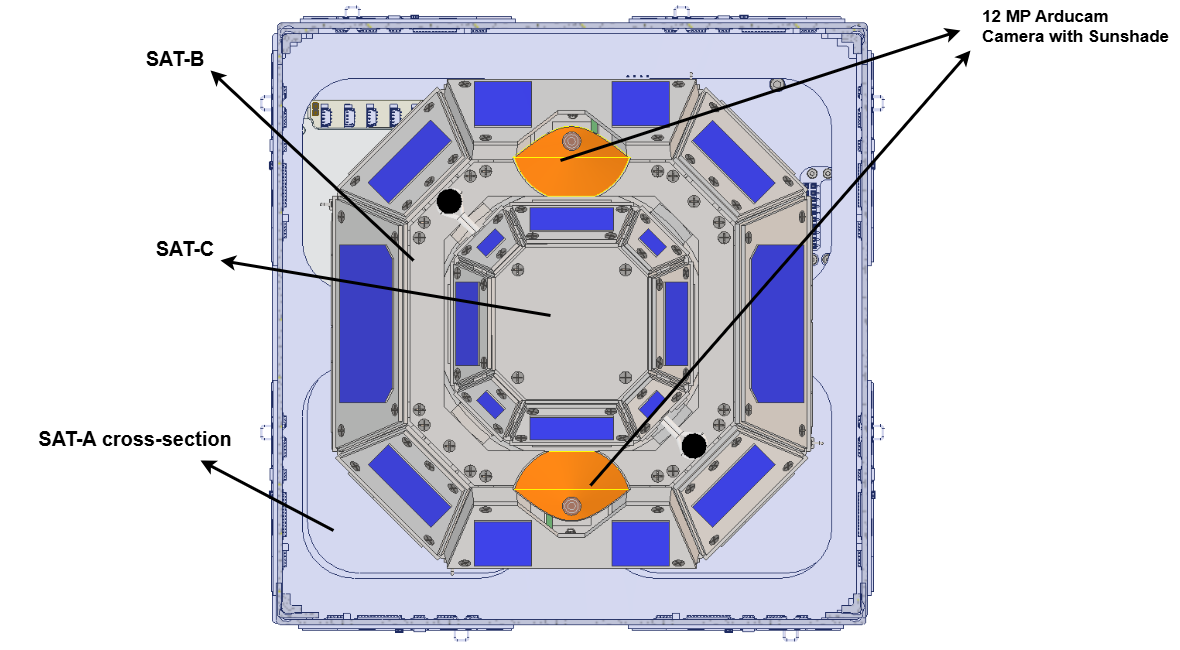
\includegraphics[
        width=0.9\linewidth,
        height=8cm,
        keepaspectratio
    ]{PUCP_pictures/Top View of the LINKU Project Assembly.png}
    \caption{Top view of the SAT-BC accommodation inside SAT-A.}
    \label{fig:linku_project_top_view}
\end{figure}

The current layout indicates that a guiding feature is required inside SAT-A to control the SAT-BC release path. The guide is intended to reduce the risk of contact between SAT-BC and the internal walls of SAT-A during ejection, especially under the impulse generated by the deployment platform. The detailed geometry of this guide and the release clearances will be refined together with the SAT-A structure and the SAT-BC deployment interface.

This chapter defines the system-level physical configuration used in the report. The detailed tether experiment, deployment mechanism, instrumentation, communications links, ADCS functions, and structural design are described in their corresponding chapters and sections.